\graphicspath{{chapt_dutch/}{intro/}{chapt2/}{chapt3/}{chapt4/}{chapt5/}{chapt6/}{chapt7/}}

% Header
\renewcommand\evenpagerightmark{{\scshape\small Appendix A}}
\renewcommand\oddpageleftmark{{\scshape\small A data acquisition software for VME CAEN TDCs}}

\renewcommand{\bibname}{References}

\hyphenation{}

\chapter[A data acquisition software for CAEN VME TDCs]%
{A data acquisition software for CAEN VME TDCs}
\label{app1}

Certifying detectors in the perspective of HL-LHC required to develop tools for the GIF++ experiment. Among them was the \acf{DAQ} software that allows to make the communications in between the computer and the TDC modules in order to retrieve the RPC data~\cite{GIFDAQ}. In this appendix, details about the software, as of how the software was written, how it functions and how it can be exported to another similar setup.

\section{Description of the setup}
\label{app1:sec:setup}

    The CMS RPC setup at GIF++ counts 5 V1190A \acf{TDC} manufactured by CAEN~\cite{V1190AMUT}. The communication between the computer and the TDCs to transfer data is done via a V1718 VME master module also manufactured by CAEN and operated from a USB port~\cite{V1718MUT}. These VME modules are hosted into a 6U VME 6021 powered crate manufactured by W-Ie-Ne-R than can accomodate up to 21 VME bus cards~\cite{6U6000MUT}. These 3 components of the DAQ setup are shown in Figure~\ref{fig:DAQSetup}.
    
    \begin{figure}[H]
        \begin{subfigure}{0.5\linewidth}
		    \centering
			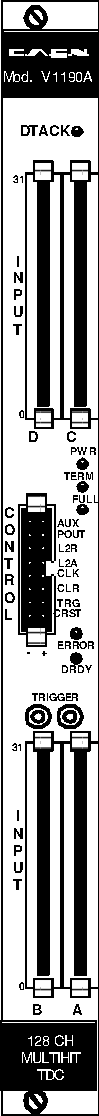
\includegraphics[height = 12cm]{fig/app1/V1190A-front.pdf}
			\caption{\label{fig:DAQSetup:A}}
		\end{subfigure}
		\begin{subfigure}{0.5\linewidth}
		    \centering
			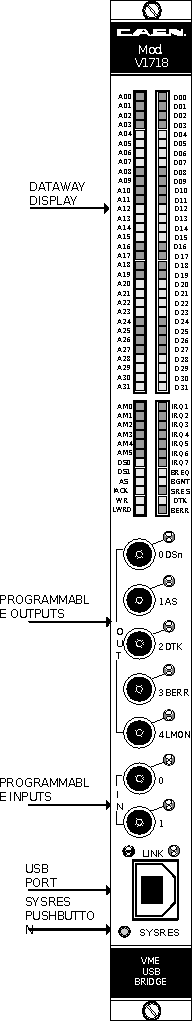
\includegraphics[height = 12cm]{fig/app1/V1718-front.pdf}\\
			\caption{\label{fig:DAQSetup:B}}
		\end{subfigure}
		\begin{subfigure}{\linewidth}
		    \centering
			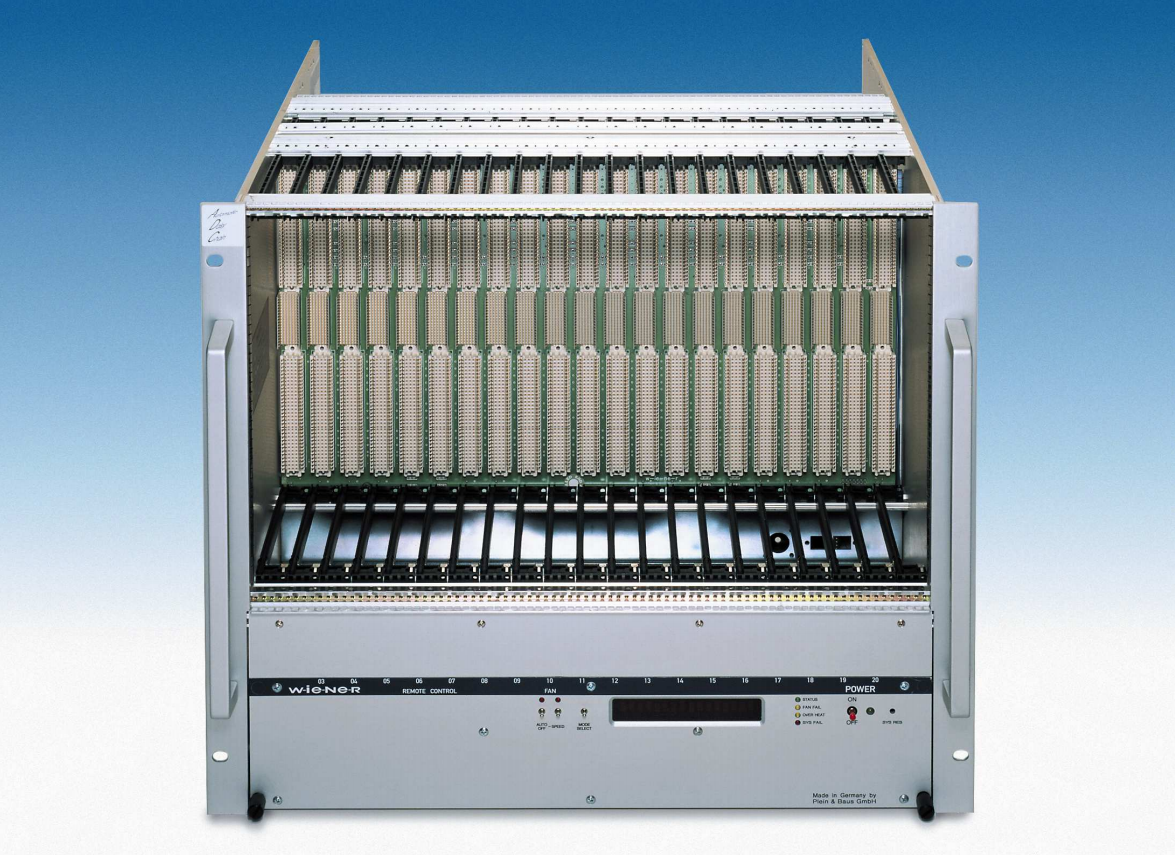
\includegraphics[width = 0.8\plotwidth]{fig/app1/Wiener-front.png}
			\caption{\label{fig:DAQSetup:C}}
		\end{subfigure}
		\caption{\label{fig:DAQSetup} (\ref{fig:DAQSetup:A}) View of the front panel of a V1190A TDC module~\cite{V1190AMUT}. (\ref{fig:DAQSetup:B}) View of the front panel of a V1718 Bridge module~\cite{V1718MUT}. (\ref{fig:DAQSetup:C}) View of the front panel of a 6U 6021 VME crate~\cite{6U6000MUT}.}
	\end{figure}

\section{Data read-out}

	As previously described in Section~\ref{ssec:PulseProc}, CMS RPC FEEs provide us with \SI{100}{ns} long LVDS output signals that are injected into the TDCs' input. V1190A are VME units accepting 128 independent Multi-Hit/Multi-Event TDC channels whose signals are treated by 4 \SI{100}{ps} high performance TDC chips developped by CERN/ECP-MIC Division. The DAQ used at GIF takes profit of the \textit{Trigger Matching Mode} offered by V1190A modules. A trigger matching is performed in between a trigger time tag and the channel time measurements. Control over this data acquisition mode, explained through Figure~\ref{fig:V1190A-TMM}, is offered through 4 programmable parameters:
        
	\begin{itemize}
		\item \textbf{match window:} the match between a trigger and a hit is done within a programmable time window
		\item \textbf{window offset:} temporal distance between the trigger tag and the start of the trigger matching window
		\item \textbf{extra search margin:} an extended time window is used to ensure that all matching hits are found
		\item \textbf{reject margin:} older hits are automatically rejected to preven buffer overflows and to speed up the search time
	\end{itemize}
    
    \begin{figure}[H]
		\centering
		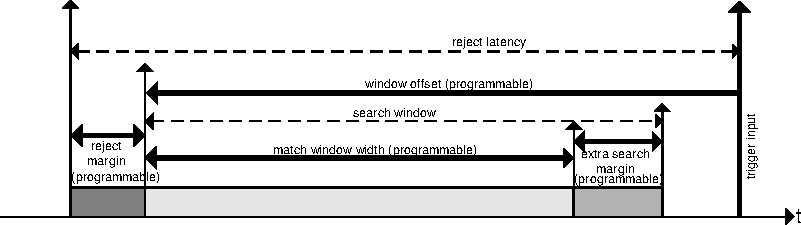
\includegraphics[width = 1.25\plotwidth]{fig/app1/V1190A-TMM.pdf}\\
		\caption{\label{fig:V1190A-TMM} Module V1190A \textit{Trigger Matching Mode} timing diagram~\cite{V1190AMUT}.}
	\end{figure}
	
	During the studies performed in GIF++, both the efficiency of the RPCs, using a muon beam, and the noise or gamma background rate are monitored.
	In the first case, the signal provided by the coïncidence of scintillators when a bunch of muons passes though the area is used to trigger the data acquisition. For this measurement, it is useful to reduce the match window width only to contain the muon information. Indeed, the delay in between a trigger signal and the detection of the corresponding muon in the RPC being very contant (typically a few tens of ns due to jitter), the muon signals are very localised in time [continue pleaeaeaeaze]. Thus the settings where chosen to have a window width of \SI{600}{ns}  whereas in the second case, the triggerring signal is provided by a pulse generator to ensure that the data taking occurs in a random way to probe only the irradiation spectrum on the detectors.

\section{Software export}


\clearpage{\pagestyle{empty}\cleardoublepage}
